\section{Dataset}

\subsection{Data Aquisition}

The self-designed imaging device for acquiring hand images \cite{hao2008multispectral,hao2007comparative} is shown in Figure \ref{fig:device_architecture}. The device operates in a contact-free environment, during the imaging process:
\begin{enumerate}
    \item Illumination Setup:
        \begin{itemize}
            \item The device uses six groups of LEDs with wavelengths ranging from violet to near-infrared. These LEDs are turned on sequentially, allowing a time-division strategy for acquiring multispectral images.
            \item This setup ensures the acquisition of images under varying illumination conditions, covering different layers of the skin due to light absorption and scattering properties.
        \end{itemize}
    \item Reflective Imaging:
        \begin{itemize}
            \item Images are captured in a reflective manner under a sheltered environment, ensuring consistent illumination and reducing external noise.
            \item Each group of LEDs is arranged circularly and diffused using a ground glass to provide even illumination across the hand.
        \end{itemize}
    \item Contact-Free Operation:
        \begin{itemize}
            \item Subjects are instructed to naturally stretch their hands, palms facing the camera, without any physical contact with a tangible surface or plate. This setup enhances hygiene and minimizes user resistance.
        \end{itemize}
    \item Sequential Image Capture:
        \begin{itemize}
            \item A single camera is used to sequentially capture images under each spectral light. This time-division strategy improves scalability and offers a better performance-to-cost ratio compared to frequency-division methods requiring multiple cameras.
        \end{itemize}
\end{enumerate}

The design allows for a detailed capture of both superficial and subsurface skin structures, revealing features like principal lines and blood vessels, which are critical for biometric analysis.

\begin{figure}[H]
    \centering
    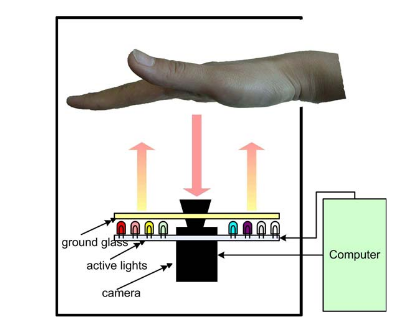
\includegraphics[width=0.5\textwidth]{./images/device-architecture.png}
    \caption{Imaging Device Architecture for Hand Image Acquisition.}
    \label{fig:device_architecture}
\end{figure}

\subsection{Dataset Description}

The CASIA Multi-Spectral Palmprint Image Database consists of 7,200 palm images captured from 100 individuals using a self-designed multispectral imaging device. The images are 8-bit gray-level JPEG files. For each hand, two sessions of palm images were captured, with a time interval of more than one month between the sessions to simulate real-world conditions and introduce natural variability. Each session includes three samples, with each sample containing six palm images captured simultaneously under six different electromagnetic spectrums, corresponding to wavelengths of 460 nm, 630 nm, 700 nm, 850 nm, 940 nm, and white light. Variations in hand postures were allowed between the two sessions to increase the diversity of intra-class samples, thereby simulating practical usage scenarios and enhancing the robustness of biometric recognition systems trained on this dataset.

\begin{figure}[H]
    \centering
    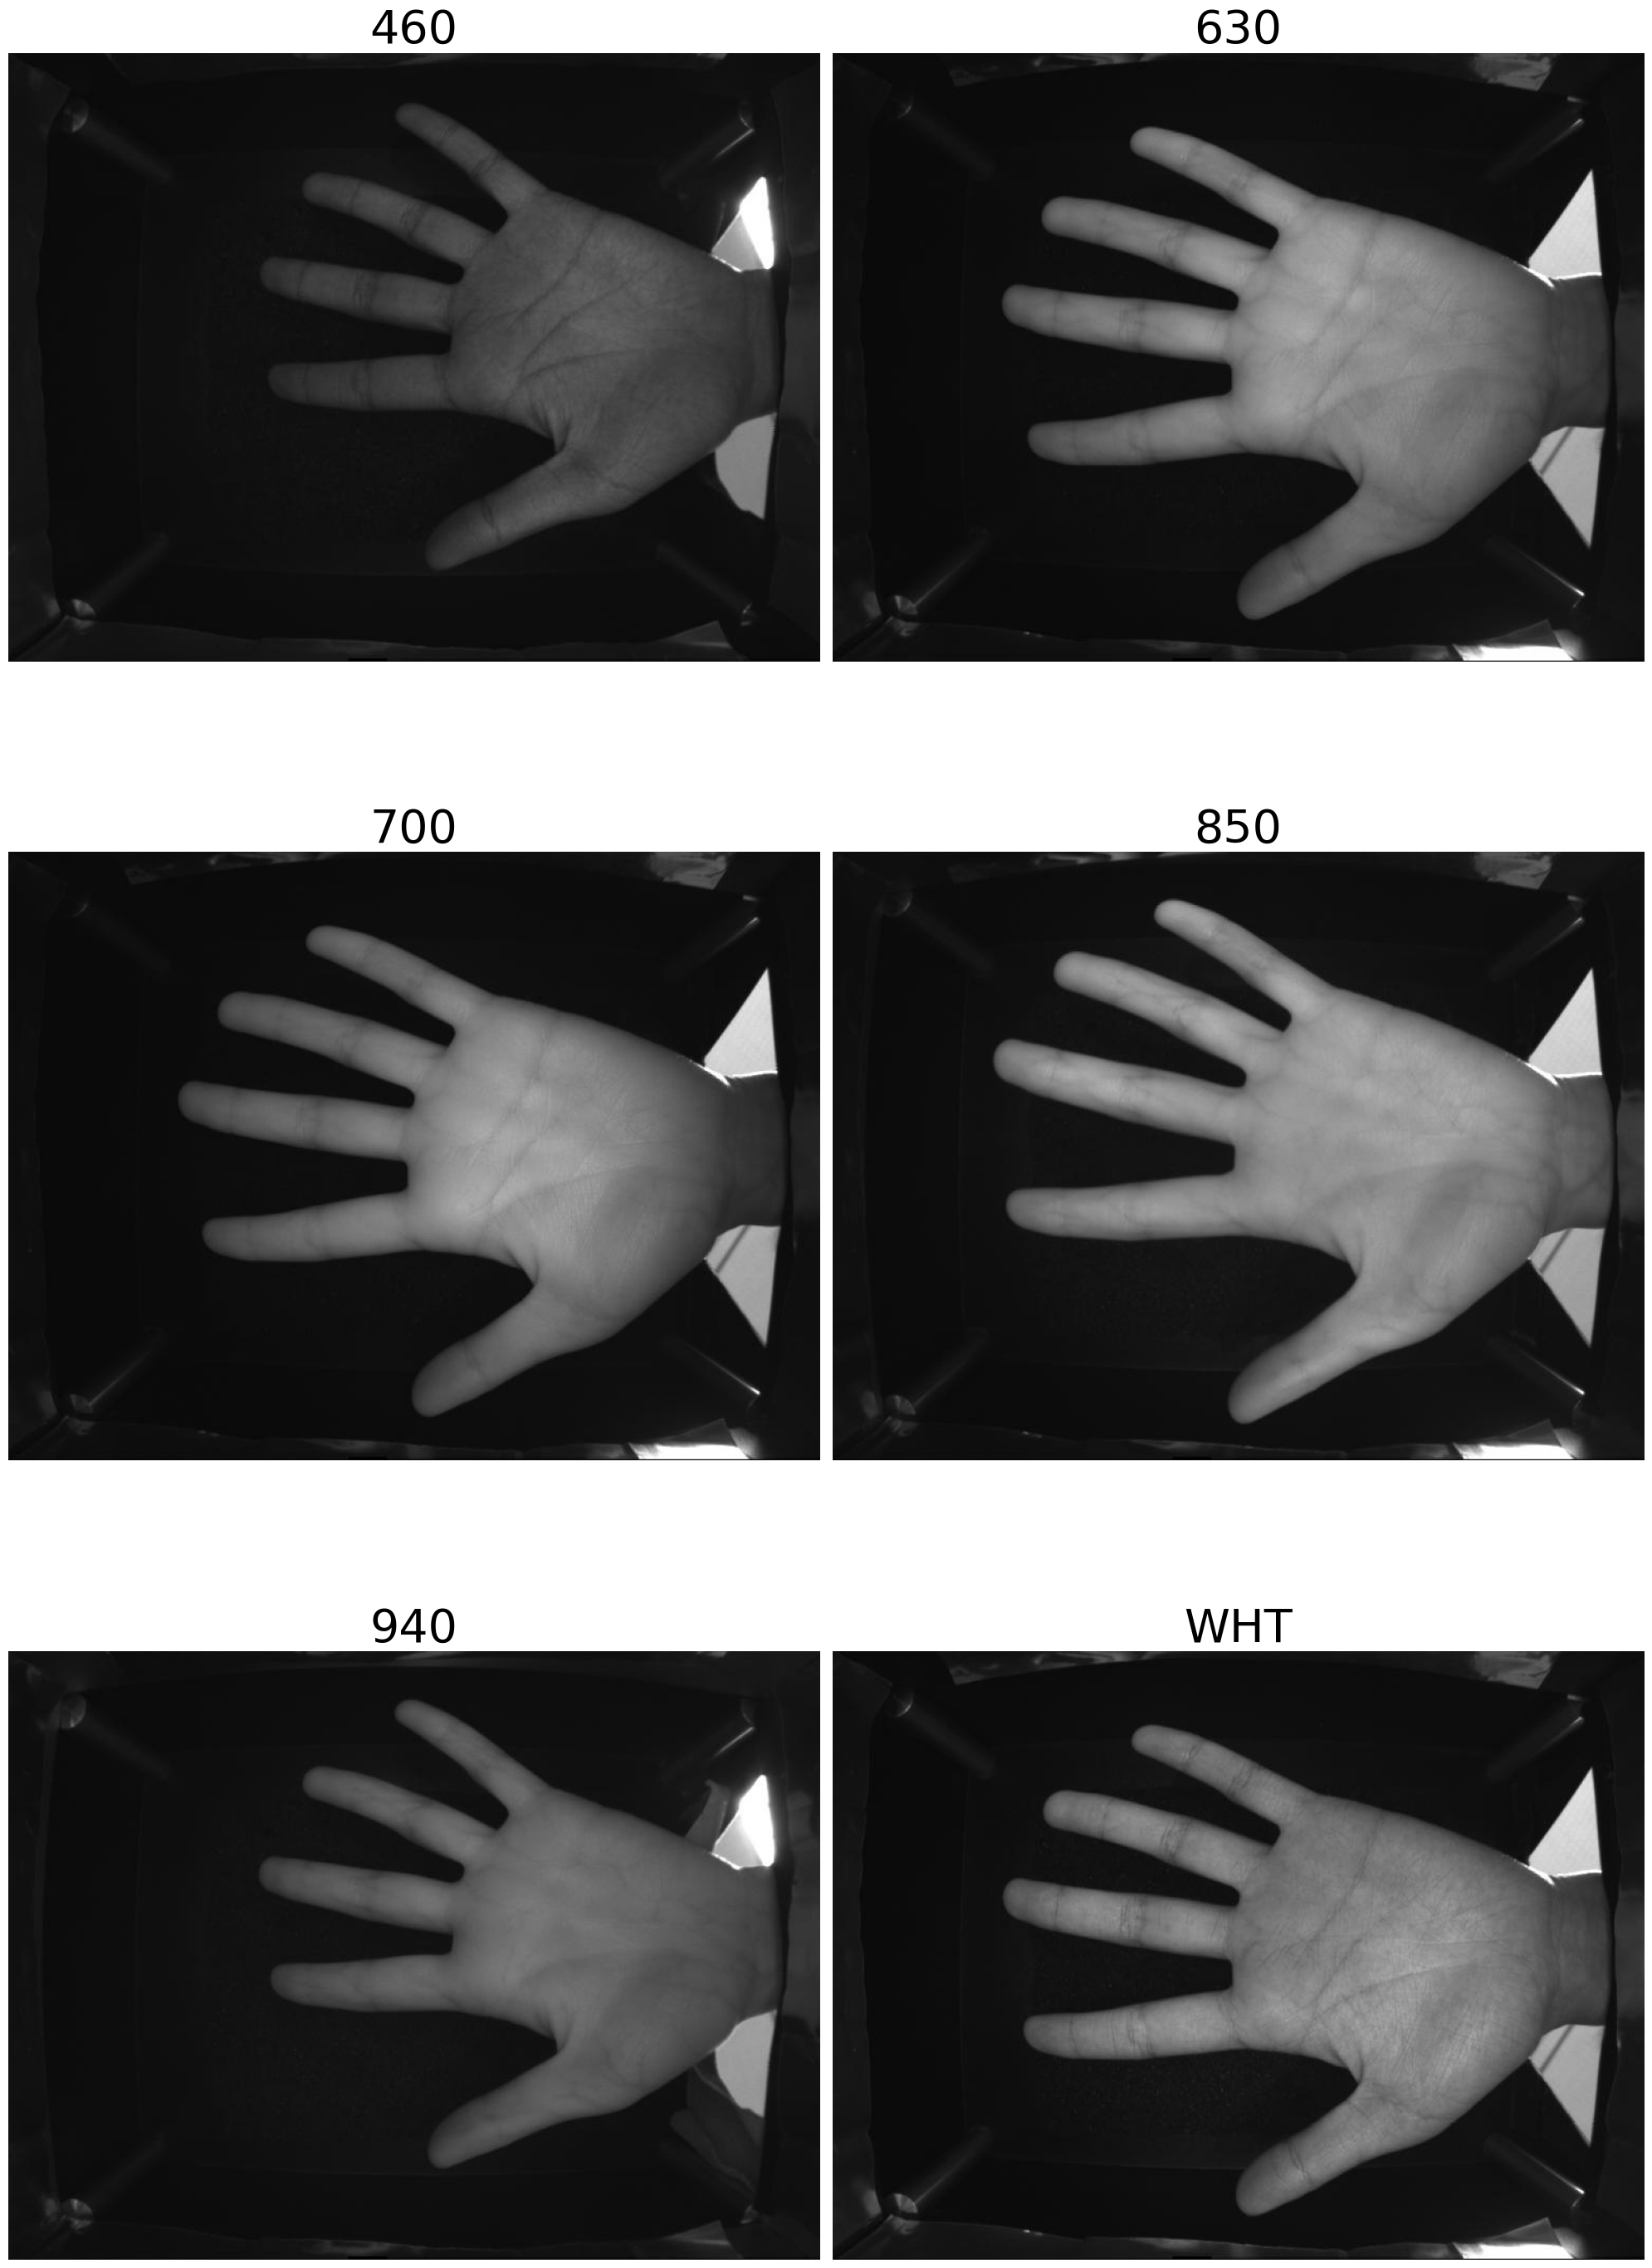
\includegraphics[width=0.5\textwidth]{./images/spectrums.png}
    \caption{Palmprint images from the CASIA Multi-Spectral Palmprint Image Database with the six spectral bands. Starting from the top-left corner and moving clockwise: 460 nm, 630 nm, 700 nm, 850 nm, 940 nm, and white light.}
    \label{fig:dataset_example}
\end{figure}